\documentclass[12pt]{article}


\usepackage{amssymb}
\usepackage{amsmath}
\usepackage{fullpage}
\usepackage{epsfig}
\usepackage{epstopdf}
\everymath{\displaystyle}
\usepackage{enumerate}

\newif\ifans

\ansfalse

\begin{document}

\begin{center}
\underline{\LARGE{Planes}}
\end{center}

\noindent SUGGESTED REFERENCE MATERIAL:

\bigskip

\noindent As you work through the problems listed below, you should reference Chapter 11.6 of the recommended textbook (or the equivalent chapter in your alternative textbook/online resource) and your lecture notes.

\bigskip

\noindent EXPECTED SKILLS:

\begin{itemize}

\item Be able to find the equation of a plane that satisfies certain conditions by finding a point on the plane and a vector normal to the plane. 

\item Know how to find the parametric equations of the line of intersection of two (non-parallel) planes. 

\item Be able to find the (acute) angle of intersection between two planes.

\end{itemize}

\noindent PRACTICE PROBLEMS:

\medskip

\begin{enumerate}

\item For each of the following, find an equation of the plane indicated in the figure.

\begin{tabular}{cccc}
(a)& & (b)&\\
&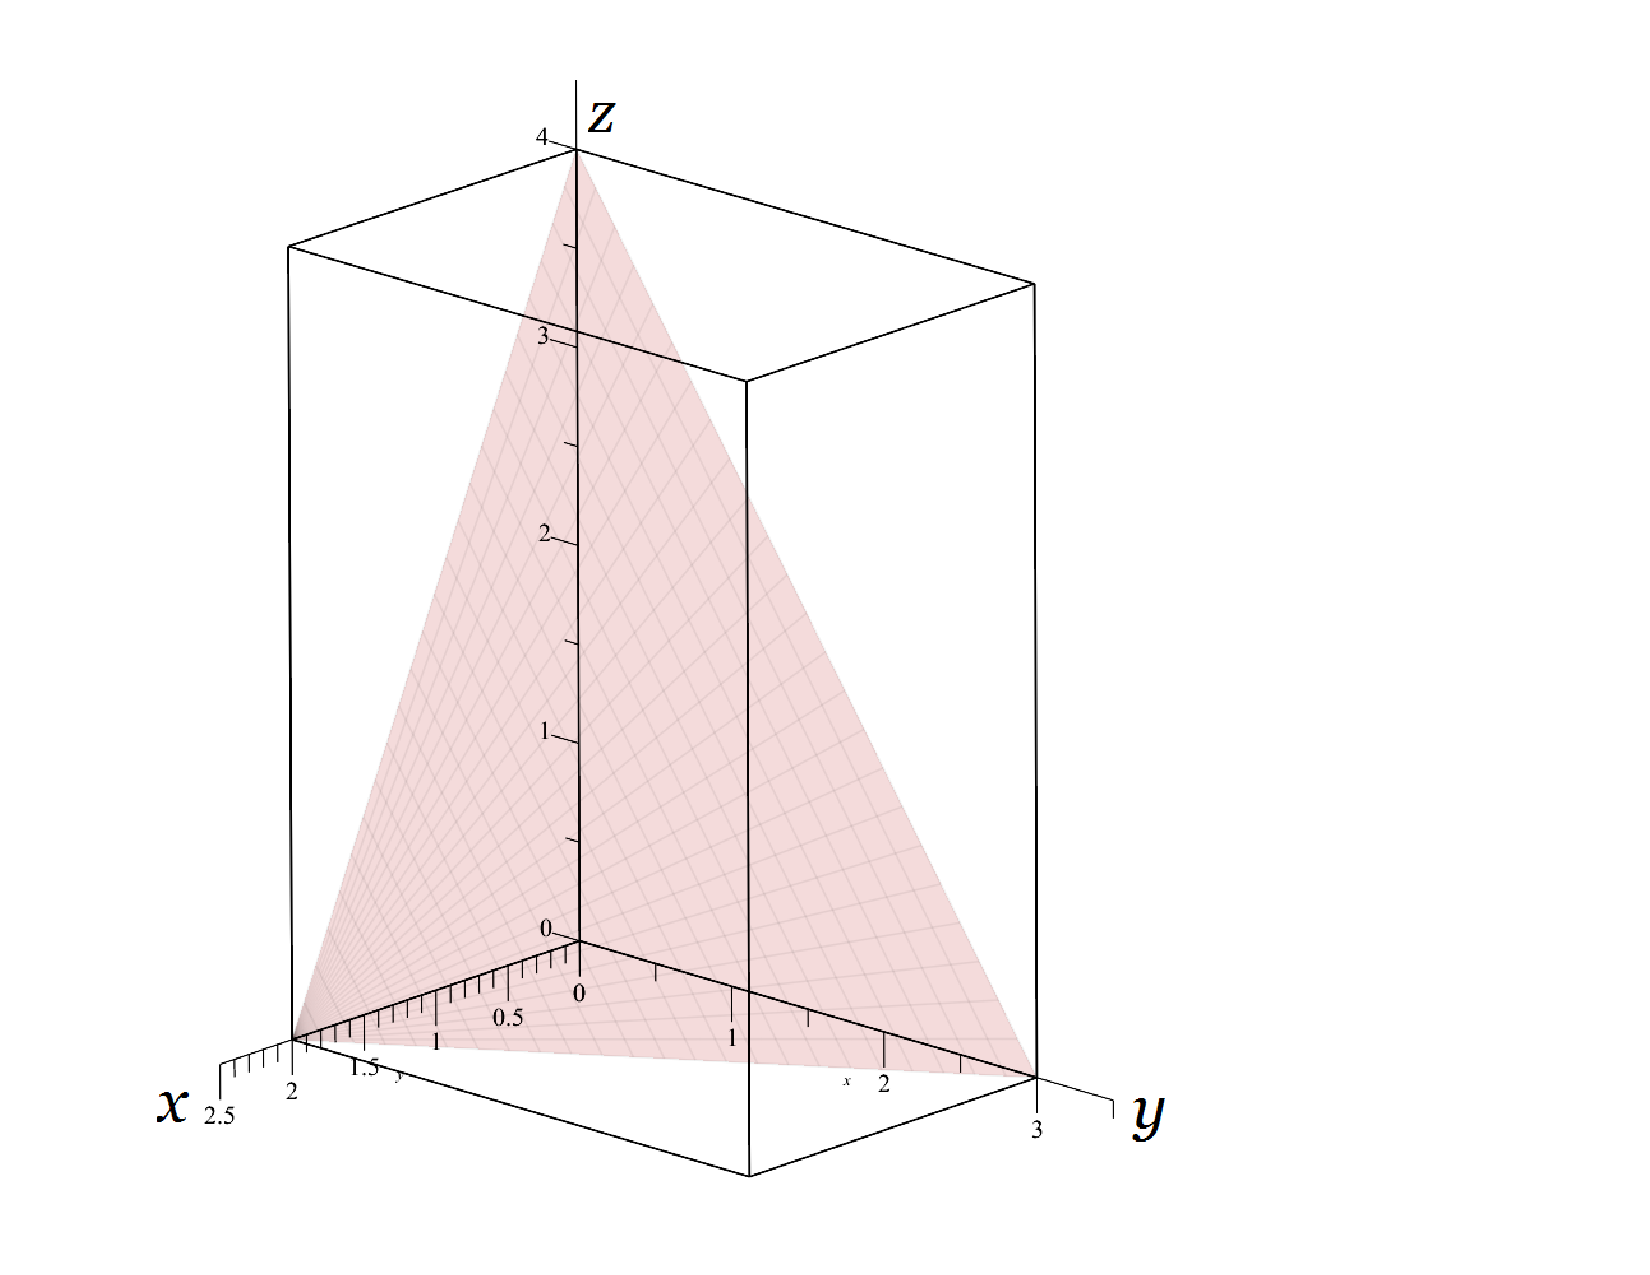
\includegraphics[scale=0.35]{plane2.pdf}&&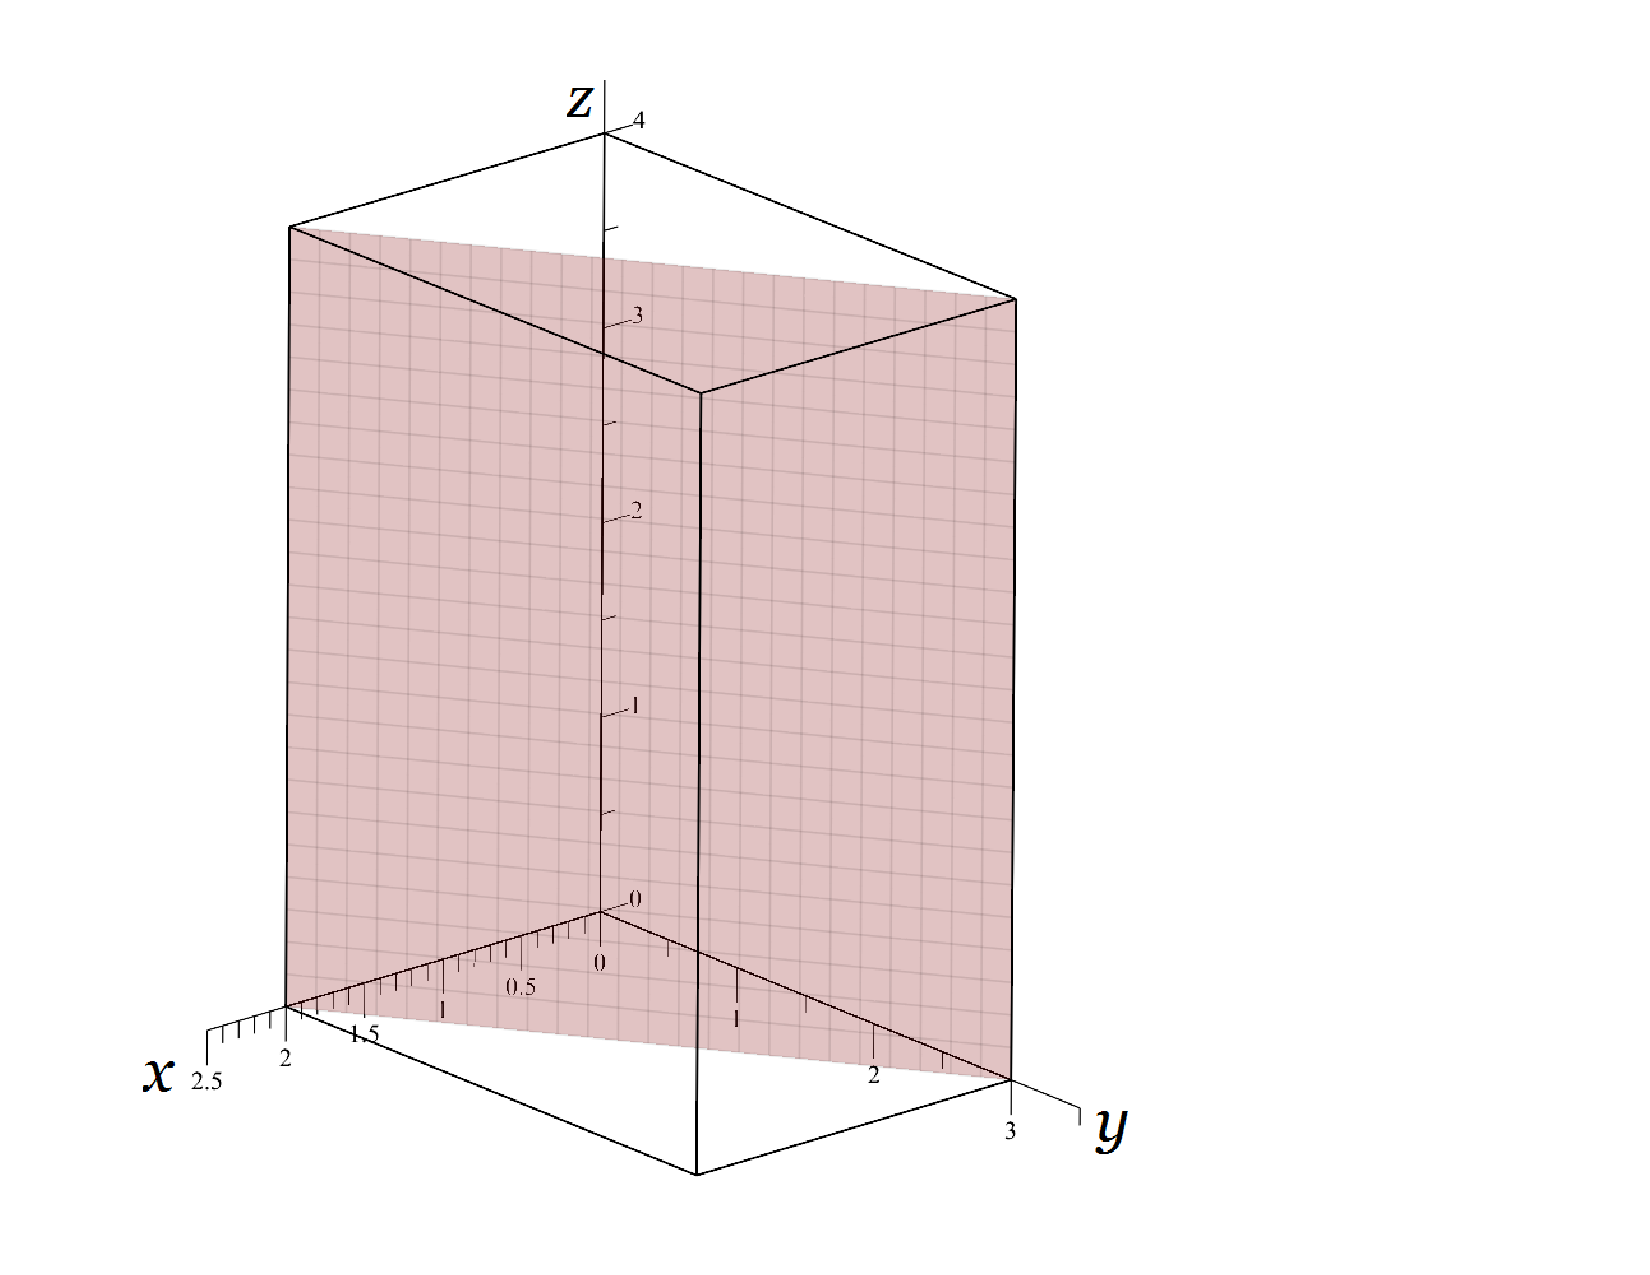
\includegraphics[scale=0.35]{plane1.pdf}
\end{tabular}

\ifans{\fbox{(a) $6x+4y+3z=12$; (b) $3x+2y=6$}} \fi

\end{enumerate}

\noindent {\bf For problems 2-6, determine whether the following are parallel, perpendicular, or neither.}

\begin{enumerate}
\setcounter{enumi}{1}

\item Plane $P_1:5x-3y+4z=-1$ and plane $P_2: 2x-2y-4z=9$

\ifans{\fbox{The planes are perpendicular.}} \fi

\item Plane $P_1: 3x-2y+z=-3$ and plane $P_2: 5x+y-6z=8$

\ifans{\fbox{The planes are neither parallel nor perpendicular.}} \fi

\item Plane $P_1: 3x-2y+z=-3$ and plane $P_2: -6x+4y-2z=1$

\ifans{\fbox{The planes are parallel.}} \fi

\item Plane $P:5x-3y+4z=-1$ and line $\overrightarrow{\ell}(t)=\left\langle2+2t, 3-2t, 5-4t\right\rangle$

\ifans{\fbox{The plane and the line are parallel.}} \fi

\item Plane $P:5x-3y+4z=-1$ and line $\overrightarrow{\ell}(t)=\left\langle2+\frac{5}{2}t, 3-\frac{3}{2}t, 5+2t\right\rangle$

\ifans{\fbox{The plane and the line are perpendicular.}} \fi

\item Give an example of a plane, $P$, and a line, $L$, which are neither parallel nor perpendicular to each other.

\ifans{\fbox{\parbox{1\linewidth}{Suppose your line has the form $\overrightarrow{\ell}(t)=\overrightarrow{\ell_0}+t\overrightarrow{v}$ and that your plane has $\overrightarrow{n}$ as a normal vector.  Then all possible answers are those for which $\overrightarrow{v} \not\parallel \overrightarrow{n}$ (i.e., $\overrightarrow{v}\neq c\overrightarrow{n}$ for any scalar $c$) and $\overrightarrow{v} \not\perp \overrightarrow{n}$ (i.e., $\overrightarrow{v}\cdot\overrightarrow{n}\neq 0$).  The first condition ensures that $L$ and $P$ are not perpendicular; the second condition ensures that $L$ and $P$ are not parallel.}}} \fi

\end{enumerate}

\noindent {\bf For problems 8-13, find an equation of the plane which satisfies the given conditions.}

\begin{enumerate}
\setcounter{enumi}{7}

\item The plane which passes through the point $P(1,2,3)$ and which has a normal vector of ${\bf n}=4{\bf i}-2{\bf j}+6{\bf k}$.

\ifans{\fbox{$4(x-1)-2(y-2)+6(z-3)=0$}} \fi

\item The plane which passes through $P(-2,0,1)$ and is perpendicular to the line $\overrightarrow{\ell}(t)=\langle 1,2,3 \rangle +t \langle 3,-2,2\rangle$.

\ifans{\fbox{$3(x+2)-2y+2(z-1)=0$}} \fi

\item The plane which passes through points $A(1,2,3)$, $B(2,-1,5)$ and $C(-1,3,3)$.

\ifans{\fbox{$-2(x-1)-4(y-2)-5(z-3)=0$}} \fi

\item The plane which passes through $A(1,2,3)$ and is parallel to the plane $3x-5y+z=2$.

\ifans{\fbox{$3(x-1)-5(y-2)+1(z-3)=0$}} \fi

\item The plane which passes through $A(-2,1,5)$ and is perpendicular to the line of intersection of $P_1: 3x+2y-z=5$ and $P_2: -y+z=7$.

\ifans{\fbox{$1(x+2)-3(y-1)-3(z-5)=0$}} \fi

\item The plane which contains the point $A(-2,-1,3)$ and which contains the line $L: x=1+t, y=3-2t, z=4t$.

\ifans{\fbox{$2(x+2)-3(y+1)-2(z-3)=0$}} \fi

\item Consider the planes $P_1: x+y+z=7$ and $P_2: 2x+4z=6$.

\begin{enumerate}

\item Compute an equation of the line of intersection of $P_1$ and $P_2$.

\ifans{\fbox{\parbox{1\linewidth}{One parametric equation of the line of intersection is $L: x=3-2t, y=4+t, z=t$}}} \fi

\item Compute an equation of the plane which passes through the point $A(1,2,3)$ and contains the line of intersection of $P_1$ and $P_2$.

\ifans{\fbox{$5(x-1)+4(y-2)+6(z-3)=0$}} \fi

\end{enumerate}

\item Find the acute angle of intersection of $P_1: 3x-2y+5z=0$ and $P_2: -x-y+2z=3$.

\ifans{\fbox{$\cos^{-1}\left(\frac{9}{\sqrt{38}\sqrt{6}}\right)$}} \fi

\item Find the acute angle of intersection of $P_1: 3x-2y-5z=0$ and $P_2: -x-y+2z=3$.

\ifans{\fbox{$\pi-\cos^{-1}\left(\frac{-11}{\sqrt{38}\sqrt{6}}\right)$}} \fi

\item Consider the plane which passes through the point $Q$ and whose normal vectors are parallel to ${\bf n}$.  And, let $P$ be another point in space, as illustrated below.

\begin{center}
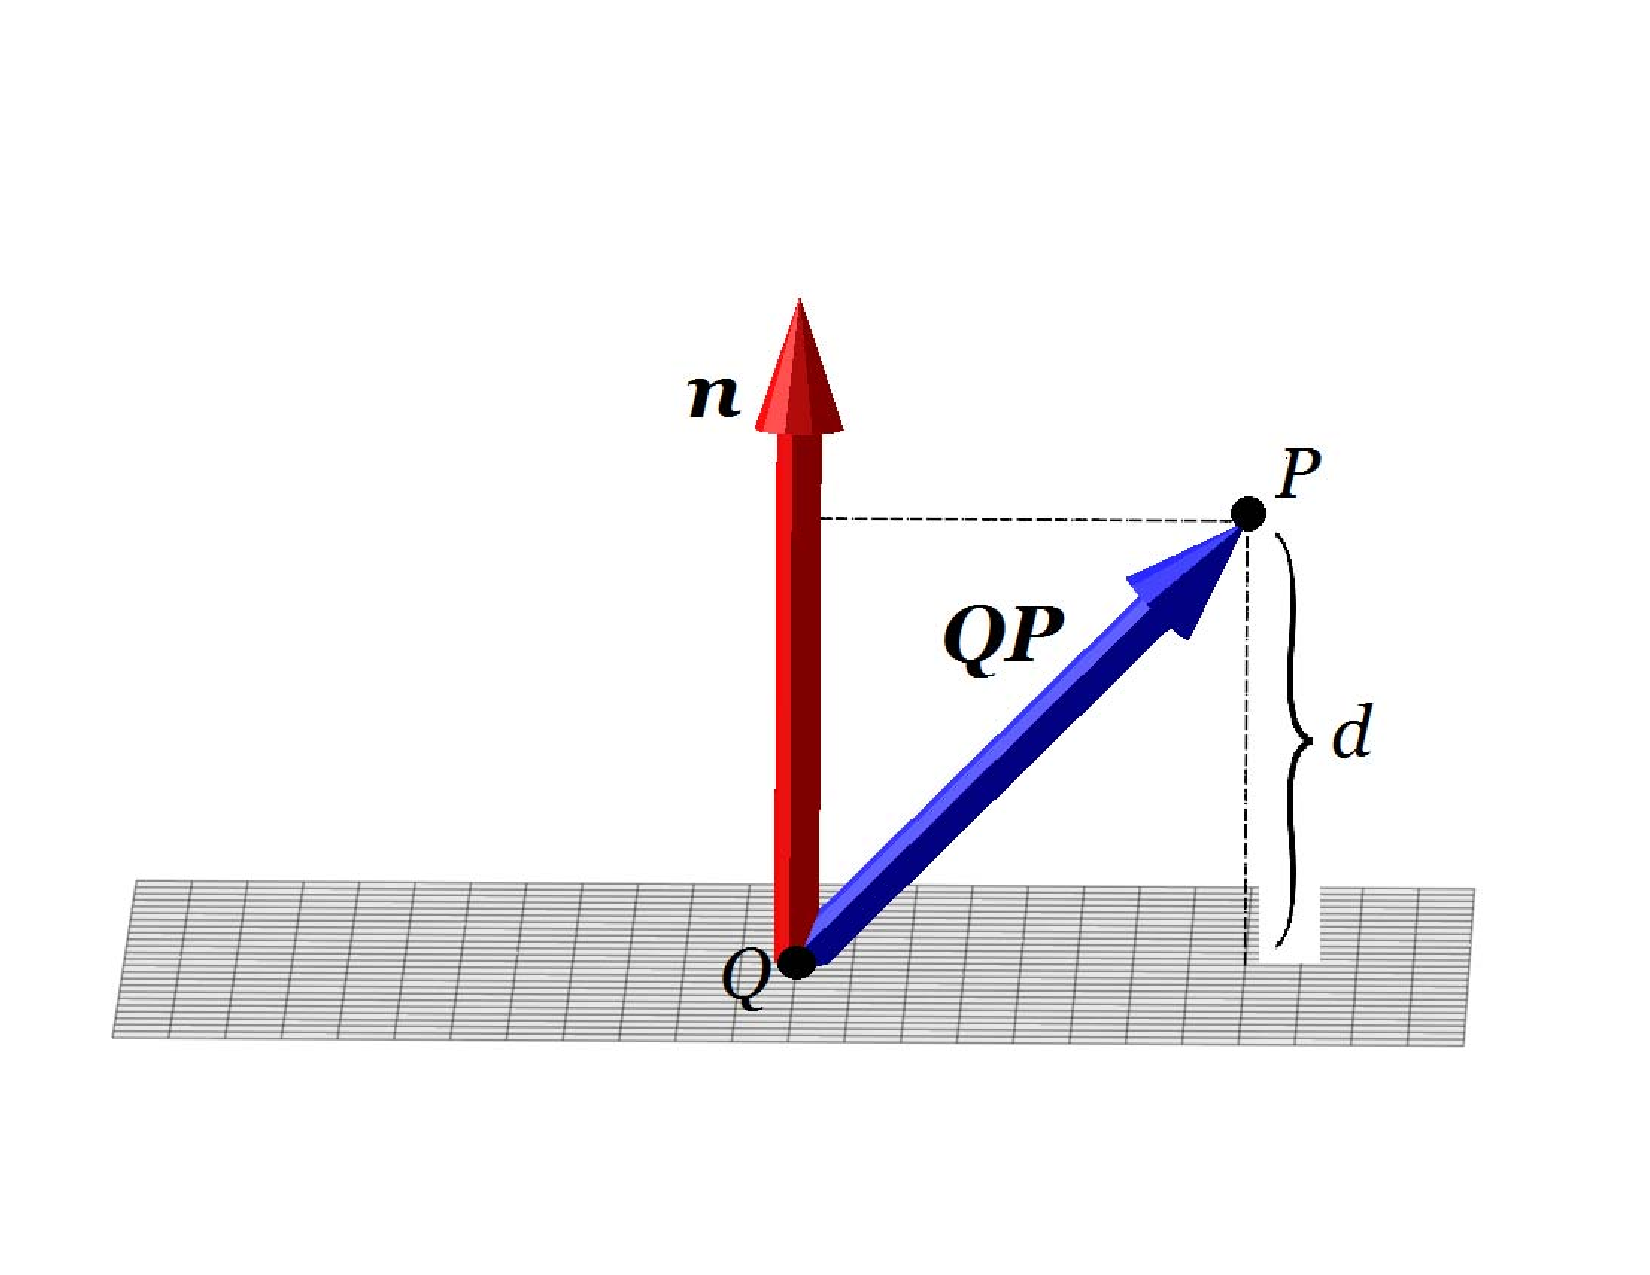
\includegraphics[scale=0.5]{distance.pdf}
\end{center}

\begin{enumerate}

\item Show that the distance between the point $P$ and the given plane is $d=\frac{|{\bf QP}\cdot{\bf n}|}{\|{\bf n}\|}$.

\ifans{\fbox{$d=\left\|\text{Proj}_{\bf n}{\bf QP}\right\|=\left\|\left(\frac{{\bf QP}\cdot{\bf n}}{\|{\bf n}\|^2}\right){\bf n}\right\| =\frac{|{\bf QP}\cdot{\bf n}|}{\|{\bf n}\|^2}\|{\bf n}\|=\frac{|{\bf QP}\cdot {\bf n}|}{\|{\bf n}\|}$}} \fi

\item Use this method to compute the distance between the point $P(2,-1,4)$ and the plane $x+2y+3z=5$.

\ifans{\fbox{$d=\frac{7}{\sqrt{14}}$}} \fi

\end{enumerate}

\item Consider planes $P_1:2x-4y+5z=-2$ and $P_2:x-2y+\frac{5}{2}z=5$.

\begin{enumerate}

\item Verify that $P_1$ and $P_2$ are parallel.

\ifans{\fbox{\parbox{1\linewidth}{${\bf n_1}=\langle 2, -4, 5\rangle$ is normal to plane $P_1$.\\
${\bf n_2}=\left\langle 1, -2, \frac{5}{2}\right\rangle$ is normal to plane $P_2$.\\
Since ${\bf n_1}=2{\bf n_2}$, we have that ${\bf n_1}$ and ${\bf n_2}$ are parallel.  And, because these normal vectors are parallel, the planes $P_1$ and $P_2$ are parallel, too.}}} \fi

\item Compute the distance between $P_1$ and $P_2$.  (Hint: See the previous problem.)

\ifans{\fbox{$d=\frac{12}{\sqrt{45}}$}} \fi

\end{enumerate}

\end{enumerate}

\end{document}